%%%%%%%%%%%%%%%%%%%%%%%%%%%%%
%Update: <Sep/24/2010>
%%%%%%%%%%%%%%%%%%%%%%%%%%%%%
\chapter{マイクロコンピュータ応用}

\section{目的}

今回は, 前学期のマイクロコンピュータ基礎で行ったアセンブリ言語の復習を行います。今回
復習するのは, データの転送, ループ, 条件分岐, LEDの制御です。

\section{装置}

前学期で用いたマイコントレーナMT-Zを用いる。

\section{実験 }

今回は, 前学期習ったZ80アセンブリを復習します。アセンブリプログラミングで必要な
ニーモニックは, 付属のニーモニッ
クと機械語のリストに機能と機械語が記載されているので, 参考にしてください。

\subsection{レジスタ, メモリの操作の復習}


レジスタとメモリはデータを保存する場所です。ここでは, レジスタやメモリのデータ
の転送の仕方を復習します。

\begin{description}



\item[課題1] 8500Hの数値に5を足した数値を, 8501Hに書き込むプログラムを作りなさい(\tabref{tab:q1-1})。

\begin{itemize}
\item データを転送するニーモニックは``LD''を使います。``LD''はデータを
任意の場所へ送る命令です。基本的な使い方は, ``LD データの転送先,
データの転送元''です。

\item 加算を行うニーモニックは``ADD''です。
\end{itemize}


\begin{table}
\begin{center}
\caption{課題1のプログラム}
\label{tab:q1-1}
\small
\begin{tabular}{|c|l|l|l|}
\hline
アドレス& \multicolumn{1}{|c|}{機械語}&\multicolumn{1}{|c|}{ニーモニック}&\multicolumn{1}{|c|}{コメント}\\
\hline
   8400&             &       ORG 8400H     &\\
   8400&   \underline{~~~~} \underline{~~~~} \underline{~~~~}  &        LD A,
            (8500H)& 8500Hの値をAレジスタに転送\\
   8403&   \underline{~~~~} \underline{~~~~}     &        ADD A, 05H&Aレジスタの
                値に5を足す\\
   8405&   \underline{~~~~} \underline{~~~~} \underline{~~~~}  &        LD
            (8501H), A& Aレジスタの値を8501Hに転送\\
   8408&   \underline{~~~~} \underline{~~~~} \underline{~~~~}  &        JP
            0000H& モニタプログラムにジャンプ\\
       &             &       &\\
   8500&             &         ORG 8500H&\\
   8500&   \underline{~~~~}        &        DB 01H&\\
   8501&             &        END&\\
\hline
\end{tabular}
\end{center}
\end{table}



\item[課題2] \figref{fig:flow1}を参考に, 8500Hと8501Hの数値を足した数値を8502Hに書き込むプログラムを作りなさい。


\begin{figure}[htbp]
\begin{center}
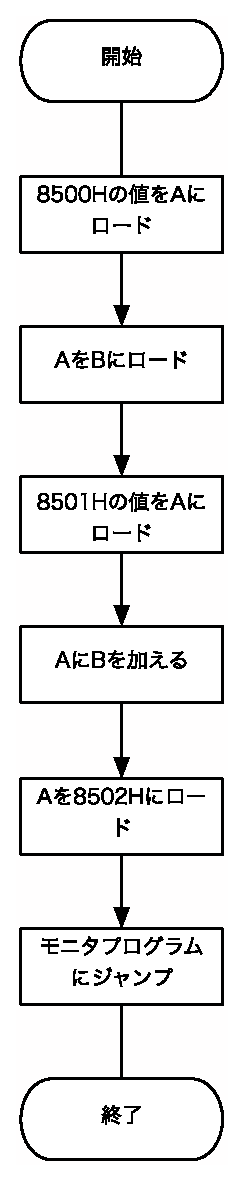
\includegraphics[height=0.6\linewidth]{img/flow1.eps}
\caption{課題2の処理の流れ。}
\label{fig:flow1}
\end{center}
\end{figure}
\end{description}

\subsection{条件分岐, ループ}

プログラミング言語として最も重要な機能の一つが条件分岐やループです。ここではアセ
ンブリにおける条件分岐, ループを復習します。

\begin{description}
\item[課題3] 8500Hと8501Hの数値を比較し, 大きい方を8502Hに書き込むプログラムを作りなさ
      い(\tabref{tab:q1-3})。


\begin{itemize}
\item データを比較するときには``CP''を使います。
比較した結果はフラグレジスタに保存されます。

\item プログラムの任意の場所にジャンプするときは``JP''を用います。
``JP 番地''で無条件に任意の番地にジャンプし, ``JP X 番地''で
フラグレジスタがXの時に任意の番地にジャンプします。
\end{itemize}


\begin{table}
\begin{center}
\caption{課題3のプログラム}
\label{tab:q1-3}
\small
\begin{tabular}{|c|l|ll|l|}
\hline
アドレス& \multicolumn{1}{|c|}{機械語}&\multicolumn{1}{|c}{ラベル}&\multicolumn{1}{c|}{ニーモニック}&\multicolumn{1}{|c|}{コメント}\\
\hline
   8400&             &        &ORG 8400H&\\
   8400&   \underline{~~~~} \underline{~~~~} \underline{~~~~}  &        &LD A,
                (8500H)& 8500Hの値をAレジスタに転送\\
   8403&   \underline{~~~~}        &        &LD B, A& Aレジスタの値をBレジスタに
                    転送\\
   8404&   \underline{~~~~} \underline{~~~~} \underline{~~~~}  &        &LD A,
                (8501H)& 8501Hの値をAレジスタに転送\\
   8407&   \underline{~~~~}         &        &CP B& Bと比較\\
   8408&   \underline{~~~~} \underline{~~~~} \underline{~~~~}   &        &JP P,
                MORE& フラグレジスタが正ならMOREにジャンプ\\
   840B&   \underline{~~~~}         &        &LD A, B& Bレジスタの値をAレジスタ
                    に転送\\
   840C&   \underline{~~~~} \underline{~~~~} \underline{~~~~}   &        &LD
                (8502H), A& Aレジスタの値を8502Hに転送\\
   840F&   \underline{~~~~} \underline{~~~~} \underline{~~~~}   &        &JP
                0000H& モニタプログラムにジャンプ\\
   8412&   \underline{~~~~} \underline{~~~~} \underline{~~~~}  &    MORE:&    LD
                (8502H), A& Aレジスタの値を8502Hに転送\\
   8415&   \underline{~~~~} \underline{~~~~} \underline{~~~~}   &        &JP
                0000H& モニタプログラムにジャンプ\\
       &             &        &&\\
   8500&             &        &ORG 8500H&\\
   8500&   \underline{~~~~} \underline{~~~~}      &        &DB 01H, 03H&\\
   8502&             &        &END&\\
\hline
\end{tabular}
\end{center}
\end{table}


\item[課題4] 10から1ずつ引いていき, 5以下になった場合終了するプログラムを作りな
           さい(\tabref{tab:q1-4})。


\begin{table}
\begin{center}
\caption{課題4のプログラム}
\label{tab:q1-4}
\small
\begin{tabular}{|c|l|ll|l|}
\hline
アドレス& \multicolumn{1}{|c|}{機械語}&\multicolumn{1}{|c}{ラベル}&\multicolumn{1}{c|}{ニーモニック}&\multicolumn{1}{|c|}{コメント}\\
\hline
   8400&            &         &ORG 8400H&\\
   8400&   \underline{~~~~} \underline{~~~~}    &         &LD A, 0AH& 値0AHをAレ
                    ジスタに転送\\
   8402&   \underline{~~~~}       &     LOOP:&    DEC A& Aから1を引く\\
   8403&   \underline{~~~~} \underline{~~~~}    &         &CP 05H&05Hと比較する\\
   8405&  \underline{~~~~} \underline{~~~~} \underline{~~~~}  &         &JP NZ,
                LOOP& フラグレジスタがNZならばLOOPにジャンプ\\
   8408&   \underline{~~~~} \underline{~~~~} \underline{~~~~} &         &LD
                (8500H), A& Aレジスタの値を8500Hに転送\\
   840B&  \underline{~~~~} \underline{~~~~} \underline{~~~~} &         &JP
                0000H& モニタプログラムにジャンプ\\
   840E&            &         &END&\\
\hline
\end{tabular}
\end{center}
\end{table}

\item[課題5] \figref{fig:flow2}を参考に, 1--10の和をメモリの8500H番地に書き込む
           プログラムを作りなさい。

\begin{figure}[htbp]
\begin{center}
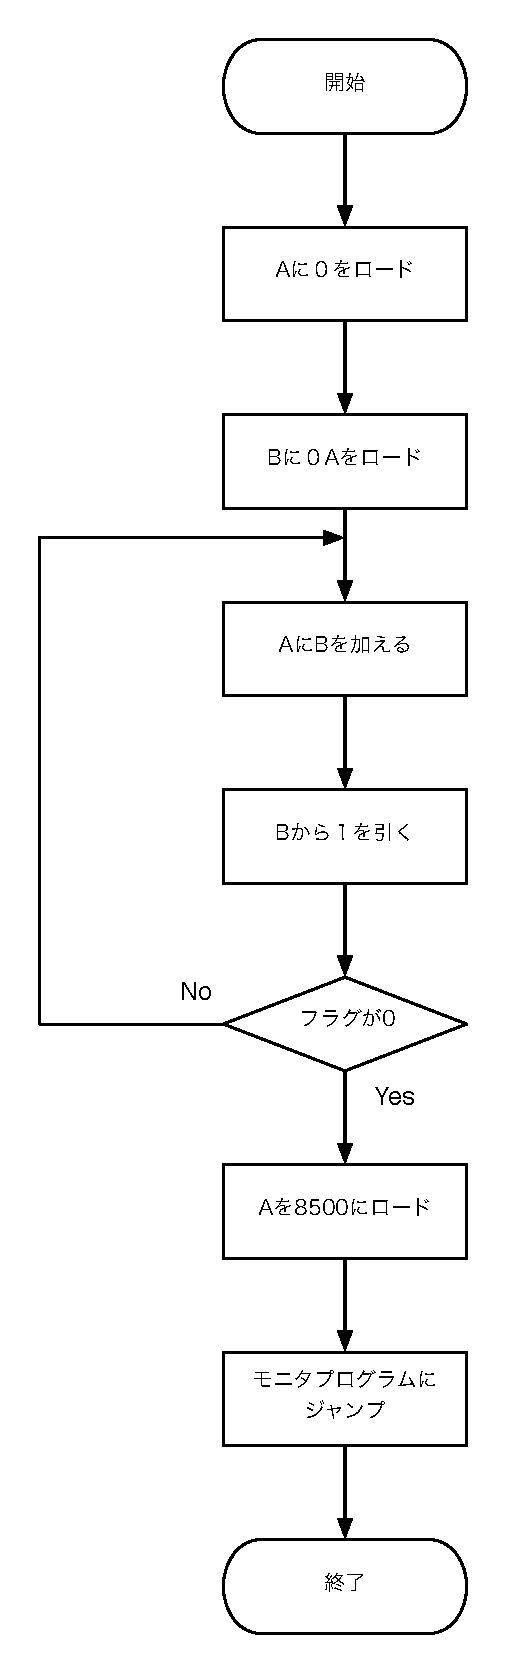
\includegraphics[width=0.2\linewidth]{img/flow2.eps}
\caption{課題5の処理の流れ}
\label{fig:flow2}
\end{center}
\end{figure}
\end{description}

\newpage

\subsection{LEDの制御の復習}

MT-Zにはパラレル入出力ICの8255Aが搭載されています。8255Aには, A, B, C, コントロー
ルのポートがあります。これらのポートを使うには, 各ポートを入
力もしくは出力で使うかの設定情報(コントロールワード)をコントロールポートに出力し
なければなりません。今回はポートAは入力, ポートB, Cは出力として使うので, コントロー
ルワードは90Hとします。
今回使うLEDはポートBにつながっています。ポートBに適切な信号を出力す
ることでLEDを制御します。

\begin{description}
\item[課題6] LEDをすべて点灯させなさい(\tabref{tab:q1-6})。

\begin{itemize}
\item ポートに信号を出力する場合は``OUT''を使います。
\end{itemize}

\begin{table}
\begin{center}
\caption{課題6の処理の流れ}
\label{tab:q1-6}
\small
\begin{tabular}{|c|l|l|l|}
\hline
アドレス& \multicolumn{1}{|c|}{機械語}&\multicolumn{1}{|c|}{ニーモニック}&\multicolumn{1}{|c|}{コメント}\\
\hline
   0005 &            &    PB EQU 05H& ポートBのアドレス\\
   0007 &            &    CTL EQU 07H& コントロールポートのアドレス\\
   0090 &            &    CLWD EQU 90H& コントロールワード\\
        &            &    &\\
   8400 &            &        ORG 8400H&\\
   8400 &  \underline{~~~~} \underline{~~~~}     &        LD A, CLWD& コントロー
                ルワードをAに転送\\
   8402 &  \underline{~~~~} \underline{~~~~}      &        OUT (CTL), A& コント
                ロールポートにAの値を出力\\
   8404 &  \underline{~~~~} \underline{~~~~} \underline{~~~~}   &        LD A,
            (8500H)& 8500Hの値をAレジスタに転送\\
   8407 &  \underline{~~~~} \underline{~~~~}     &        OUT (PB), A& ポートBにA
                を出力\\
   8409 &  \underline{~~~~} \underline{~~~~} \underline{~~~~}  &        JP
            0000H& モニタプログラムにジャンプ\\
        &            &    &\\
   8500 &            &        ORG 8500H&\\
   8500 &  \underline{~~~~}        &        DB 0FFH&\\
   8501 &            &        END&\\
\hline
\end{tabular}
\end{center}
\end{table}


\item[課題7] LEDを一つおきに点灯させなさい。

\item[課題8] LEDの点灯が反転を繰り返すプログラムを作りなさい(\tabref{tab:q1-8})。

\begin{table}
\begin{center}
\caption{課題8のプログラム}
\label{tab:q1-8}
\small
\begin{tabular}{|c|l|ll|l|}
\hline
アドレス& \multicolumn{1}{|c|}{機械語}&\multicolumn{1}{|c}{ラベル}&\multicolumn{1}{c|}{ニーモニック}&\multicolumn{1}{|c|}{コメント}\\
\hline
   0005 &            &    &PB EQU 05H& ポートBのアドレス\\
   0007 &            &    &CTL EQU 07H& コントロールポートのアドレス\\
   0090 &            &    &CLWD EQU 90H& コントロールワード\\
        &            &    &&\\
   8400 &            &    &    ORG 8400H&\\
   8400 &  \underline{~~~~} \underline{~~~~}     &    &    LD A, CLWD& コントロー
                    ルワードをAレジスタに転送\\
   8402 &  \underline{~~~~} \underline{~~~~}     &    &    OUT (CTL), A& コント
                    ロールポートにAレジスタの値を出力\\
   8404 &  \underline{~~~~} \underline{~~~~}      &    &    LD A, 08H& 値08HをA
                    レジスタに転送\\
   8406 &  \underline{~~~~} \underline{~~~~}      &    SHIFT:&     OUT (PB), A&
                    ポートBにAレジスタの値を出力\\
   8408 &  \underline{~~~~} \underline{~~~~}     &        &XOR 0FFH& Aレジスタと
                    FFHとの排他的論理和をとる\\
   840A &  \underline{~~~~} \underline{~~~~} \underline{~~~~}   &        &CALL
                TIMER& タイマを呼び出す\\
   840D &  \underline{~~~~} \underline{~~~~} \underline{~~~~}   &        &JP
                SHIFT& シフトにジャンプ\\
        &            &    &&\\
        &            &    &&\\
   8440 &            &    &    ORG 8440H&\\
   8440 &  21 00 40   &    TIMER:& LD
                HL , 4000H& 値4000HをHLレジスタに転送\\
   8443 &  5F        &    &    LD E, A&Aレジスタの値をEレジスタに
                    転送\\
   8444 &  2B        &    TLOOP:& DEC HL&HLレジスタの値から1を引く\\
   8445 &  7C        &    &    LD A, H&Hレジスタの値をAレジスタに
                    転送\\
   8446 &  B5        &    &    OR L& Aの値とLの値の論理和をとる\\
   8447 &  20 FB       &    &    JR NZ , TLOOP& フ
                    ラグレジスタがNZならばTLOOPにジャンプ\\
   8449 &  7B        &    &    LD A, E& Eレジスタの値をAレジスタに
                    転送\\
   844A &  C9        &    &    RET&ルーティンの終了\\
   844B &            &    &    END&\\

\hline
\end{tabular}
\end{center}
\end{table}


\item[課題9] \figref{fig:flow3}を参考に, LEDの点灯位置が左にシフトするプログラム
           を作りなさい。

\begin{itemize}
\item 左にシフトさせるには, 左にビットシフトさせる``RLCA''を使う。
\end{itemize}

\begin{figure}[htbp]
\begin{center}
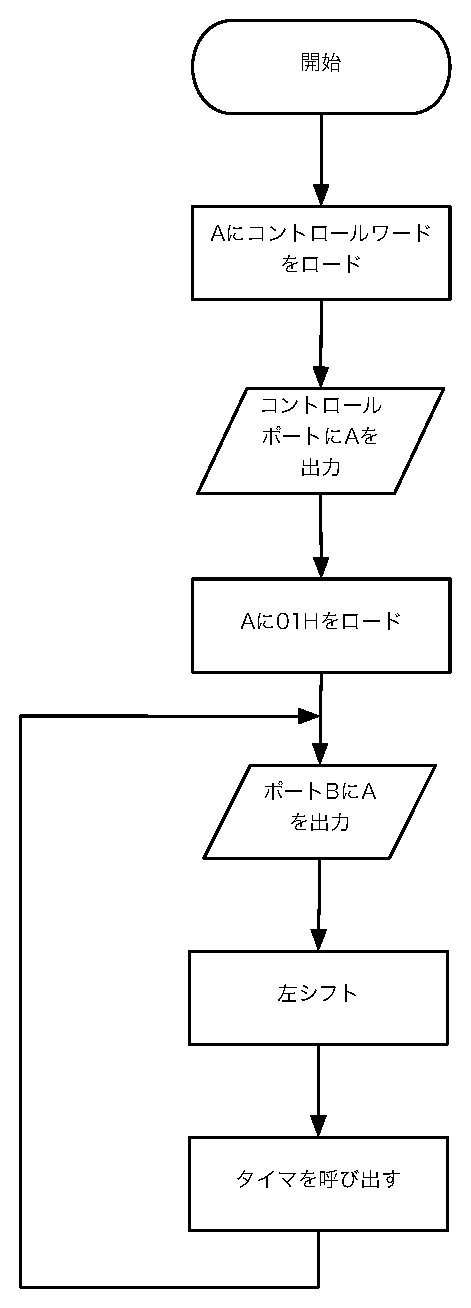
\includegraphics[width=0.4\linewidth]{img/flow3.eps}
\caption{課題9の処理の流れ}
\label{fig:flow3}
\end{center}
\end{figure}

\item[課題10(発展)] LEDの点灯位置が, 始め左にシフトし, 左端にきたら右にシフト, 右端にきたら
           左にシフトするようなプログラムを作れ。

\end{description}


\newpage
\section{考察課題}

\begin{description}
\item[考察課題1] アセンブリ言語は低級言語といわれている。低級言語とは何か報告
           しなさい。
\item[考察課題2] プログラミング言語には高級言語と呼ばれるものがある。高級言語と
           は何か報告しなさい。また, 高級言語の例を2つ報告し, その言語が主にどのような用途で使われるかなどの特
      徴も報告しなさい。

\end{description}